\documentclass[11pt,a4paper,oneside]{report}

% ============================================================================
%  DELHI PUBLIC SCHOOL INDIRAPURAM
%  OFFICIAL IT ADMINISTRATOR & OPERATIONS MANUAL
%  Comprehensive Technical Administration, Operations & Security Manual
% ============================================================================

\usepackage[utf8]{inputenc}
\usepackage[T1]{fontenc}
\usepackage{lmodern}
\usepackage[top=2.5cm, bottom=2.5cm, left=2.5cm, right=2.5cm, headheight=14pt]{geometry}
\usepackage[table]{xcolor}
\usepackage{microtype}
\frenchspacing
\usepackage{tabularx}
\usepackage{booktabs}
\usepackage{longtable}
\usepackage{array}
\usepackage{graphicx}
\usepackage{fancyhdr}
\usepackage{titlesec}
\usepackage{tocloft}
\usepackage{enumitem}
\usepackage{amsmath}
\usepackage{amssymb}
\usepackage{parskip}
\usepackage{float}
\usepackage{caption}
\usepackage{subcaption}
\usepackage{listings}
\usepackage{tikz}
\usetikzlibrary{shapes.geometric, arrows.meta, positioning, calc, backgrounds, fit}

% ── Institutional Color Palette ───────────────────────────────────────────────
\definecolor{dpsgreen}{RGB}{10, 92, 54}      % DPS Indirapuram Forest Green (#0A5C36)
\definecolor{dpsgold}{RGB}{201, 151, 42}     % Institutional Academic Gold (#C9972A)
\definecolor{dpsnavy}{RGB}{15, 32, 67}       % Deep Executive Navy (#0F2043)
\definecolor{dpsdark}{RGB}{26, 32, 44}       % Charcoal Body Dark
\definecolor{codebg}{RGB}{248, 249, 250}     % Code & Table Fill Background
\definecolor{sectioncol}{RGB}{15, 32, 67}    % Heading Section Color
\definecolor{linkblue}{RGB}{14, 116, 144}    % Deep Cyan Hyperlinks
\definecolor{alertred}{RGB}{185, 28, 28}     % Urgent / Warning Red
\definecolor{successgrn}{RGB}{22, 101, 52}   % Success / Operational Green

% ── Custom Column Types ───────────────────────────────────────────────────────
\newcolumntype{L}[1]{>{\raggedright\arraybackslash}p{#1}}
\newcolumntype{C}[1]{>{\centering\arraybackslash}p{#1}}
\newcolumntype{R}[1]{>{\raggedleft\arraybackslash}p{#1}}

% ── Header and Footer Configuration ───────────────────────────────────────────
\pagestyle{fancy}
\fancyhf{}
\fancyhead[L]{\small\textcolor{dpsnavy}{\textbf{DPS Indirapuram}} \textbar\ \textcolor{dpsgreen}{IT Administrator \& Operations Manual}}
\fancyhead[R]{\small\nouppercase{\leftmark}}
\fancyfoot[L]{\scriptsize\textcolor{gray}{CONFIDENTIAL \& PROPRIETARY --- FOR INTERNAL IT USE ONLY}}
\fancyfoot[R]{\small\thepage}
\renewcommand{\headrulewidth}{0.6pt}
\renewcommand{\footrulewidth}{0.4pt}

\fancypagestyle{plain}{
  \fancyhf{}
  \fancyfoot[L]{\scriptsize\textcolor{gray}{DPS INDIRAPURAM --- IT OPERATIONS MANUAL v3.2}}
  \fancyfoot[R]{\small\thepage}
  \renewcommand{\headrulewidth}{0pt}
  \renewcommand{\footrulewidth}{0.4pt}
}

% ── Typography & Section Styling ──────────────────────────────────────────────
\titleformat{\chapter}[display]
  {\normalfont\huge\bfseries\color{sectioncol}}
  {\chaptertitlename\ \thechapter}{12pt}{\Huge}
\titlespacing*{\chapter}{0pt}{8pt}{18pt}
\titleformat{\section}
  {\normalfont\Large\bfseries\color{sectioncol}}{\thesection}{1em}{}
\titleformat{\subsection}
  {\normalfont\large\bfseries\color{sectioncol!80}}{\thesubsection}{1em}{}
\titleformat{\subsubsection}
  {\normalfont\normalsize\bfseries\color{dpsgreen}}{\thesubsubsection}{1em}{}

% ── Code Listing Style ────────────────────────────────────────────────────────
\lstdefinestyle{admincode}{
  backgroundcolor=\color{codebg},
  basicstyle=\ttfamily\footnotesize,
  breaklines=true,
  breakatwhitespace=false,
  frame=single,
  rulecolor=\color{dpsnavy!30},
  keywordstyle=\bfseries\color{dpsgreen},
  commentstyle=\itshape\color{gray},
  stringstyle=\color{dpsgold!90!black},
  showstringspaces=false,
  tabsize=2,
  captionpos=b
}
\lstset{style=admincode}

% ── Hyperlinks & Metadata ─────────────────────────────────────────────────────
\usepackage[hyphens]{url}
\usepackage{hyperref}
\hypersetup{
  colorlinks        = true,
  linkcolor         = sectioncol,
  urlcolor          = linkblue,
  citecolor         = dpsgreen,
  bookmarks         = true,
  bookmarksnumbered = true,
  pdfstartview      = FitH,
  pdftitle          = {DPS Indirapuram -- IT Administrator and Operations Manual},
  pdfauthor         = {Lead Software Architecture Team},
  pdfsubject        = {System Operations, CMS Administration and Cybersecurity Manual},
  pdfkeywords       = {DPS Indirapuram, IT Manual, CMS Administration, Security, MongoDB, tRPC, React}
}
\pdfstringdefDisableCommands{
  \def\\{}
  \def\textbf#1{#1}
  \def\texttt#1{#1}
  \def\&{and}
}

% ── Macros ───────────────────────────────────────────────────────────────────
\newcommand{\envvar}[1]{\texttt{\textbf{\textcolor{dpsnavy}{#1}}}}
\newcommand{\rolebadge}[2]{\colorbox{#1!15}{\textcolor{#1}{\textbf{\scriptsize #2}}}}
\newcommand{\sopbox}[2]{
  \begin{center}
  \begin{minipage}{0.96\textwidth}
  \fcolorbox{dpsnavy!60}{codebg}{
    \begin{minipage}{0.96\textwidth}
    \vspace{4pt}
    \textbf{\textcolor{dpsnavy}{\large #1}}\\[4pt]
    \small #2
    \vspace{4pt}
    \end{minipage}
  }
  \end{minipage}
  \end{center}
}

% ============================================================================
%  DOCUMENT BODY
% ============================================================================
\begin{document}

% ── Title Page ────────────────────────────────────────────────────────────────
\begin{titlepage}
  \centering
  \vspace*{0.5cm}

  \IfFileExists{dpsi_crest.png}{
    
\includegraphics[height=2.8cm, keepaspectratio]{dpsi_crest.png}\\[0.4cm]
  }{
    \IfFileExists{dpsi_logo.png}{
      
\includegraphics[height=2.4cm, keepaspectratio]{dpsi_logo.png}\\[0.4cm]
    }{
      {\Large\textbf{\textcolor{dpsgreen}{DELHI PUBLIC SCHOOL INDIRAPURAM}}}\\[0.4cm]
    }
  }

  {\large\bfseries\textcolor{dpsgreen}{DELHI PUBLIC SCHOOL INDIRAPURAM}}\\[0.2cm]
  {\small\textit{Affiliated to the Central Board of Secondary Education (CBSE), New Delhi}}\\[1.0cm]

  \rule{\textwidth}{1.8pt}\\[0.4cm]
  {\fontsize{24pt}{28pt}\selectfont\bfseries\color{dpsnavy} IT ADMINISTRATOR \& OPERATIONS MANUAL}\\[0.3cm]
  {\Large\bfseries\color{dpsgold!90!black} Comprehensive Guide to Website Operations, CMS Governance, System Architecture \texorpdfstring{\&}{and} Cybersecurity Runbooks}\\[0.3cm]
  \rule{\textwidth}{1.8pt}\\[1.2cm]

  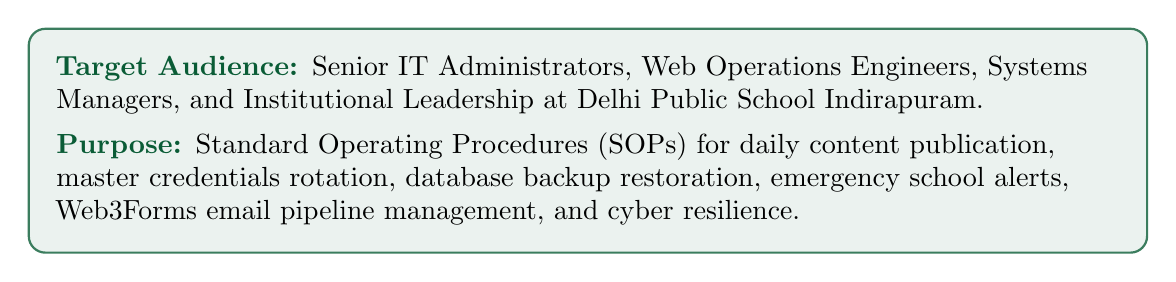
\begin{tikzpicture}
    \node[rectangle, rounded corners=6pt, draw=dpsgreen!80, fill=dpsgreen!8, thick, inner sep=10pt, text width=13.5cm, align=left] {
      \textbf{\textcolor{dpsgreen}{Target Audience:}} Senior IT Administrators, Web Operations Engineers, Systems Managers, and Institutional Leadership at Delhi Public School Indirapuram.\\[4pt]
      \textbf{\textcolor{dpsgreen}{Purpose:}} Standard Operating Procedures (SOPs) for daily content publication, master credentials rotation, database backup restoration, emergency school alerts, Web3Forms email pipeline management, and cyber resilience.
    };
  \end{tikzpicture}

  \vfill

  \begin{tabularx}{0.88\textwidth}{l X}
    \textbf{Document Version:}    & 3.2 (Production Stable) \\
    \textbf{Classification:}      & \textbf{\textcolor{alertred}{RESTRICTED --- INTERNAL IT OPERATIONS ONLY}} \\
    \textbf{Target Platform:}     & Delhi Public School Indirapuram Institutional Portal \& CMS \\
    \textbf{Core Technologies:}   & React 19, TypeScript 5.8, Hono 4, tRPC v11, MongoDB Atlas, Cloudinary, Web3Forms \\
    \textbf{Lead Author:}         & Lead Software Architect \& Engineering Operations \\
    \textbf{Effective Date:}      & Academic Session 2026--2027 \\
  \end{tabularx}

  \vspace*{0.8cm}
\end{titlepage}

% ── Table of Contents ────────────────────────────────────────────────────────
\tableofcontents
\newpage

% ============================================================================
%  CHAPTER 1 — EXECUTIVE OVERVIEW & IT RESPONSIBILITIES
% ============================================================================
\chapter{Executive Overview \texorpdfstring{\&}{and} IT Responsibilities}

\section{Mission Statement of School IT Operations}

The Delhi Public School Indirapuram (DPSI) digital ecosystem serves as the primary gateway
for prospective parents, enrolled students, faculty members, regulatory authorities (CBSE),
and the global educational community. The platform unites high-performance web engineering,
photorealistic 3D spatial tours, dynamic bilingual search, AI-assisted admissions guidance,
and an enterprise-grade administrative Content Management System (CMS).

The primary objective of the IT Administrator is to ensure \textbf{99.99\,\% uptime},
flawless data integrity, prompt communication during institutional emergencies,
and strict compliance with national data privacy standards (Digital Personal Data
Protection Act, 2023) and CBSE digital disclosure mandates.

\section{Core Responsibilities of the IT Administrator}

The IT Administrator's daily and periodic responsibilities encompass five core pillars:

\begin{enumerate}[leftmargin=*]
  \item \textbf{Content \& Announcement Governance:} Authoring, approving, and publishing
        circulars, news announcements, event galleries, and emergency closure tickers.
  \item \textbf{Admissions \& Lead Pipeline Supervision:} Monitoring real-time parent
        applications, tracking inquiry statuses, validating Web3Forms email delivery,
        and exporting applicant logs to school ERP systems.
  \item \textbf{Access Control \& Identity Governance:} Managing administrator logins,
        enforcing multi-factor hygiene, rotating secret keys, and monitoring the
        immutable security audit logs for unauthorized intrusion attempts.
  \item \textbf{Infrastructure \& Database Maintenance:} Monitoring MongoDB Atlas connection
        pools, verifying automated snapshot backups, executing point-in-time recovery,
        and optimizing Cloudinary/R2 media asset budgets.
  \item \textbf{Cybersecurity \& Disaster Recovery:} Enforcing rate limits, auditing SSL/TLS
        certificates, applying security patches, and executing standard operating procedures
        during school contingencies.
\end{enumerate}

\section{System Architecture Overview}

Figure~\ref{fig:it-architecture} illustrates the top-level operational flow across the
client presentation tier, the serverless edge execution engine, and persistent storage.

\begin{figure}[H]
\centering
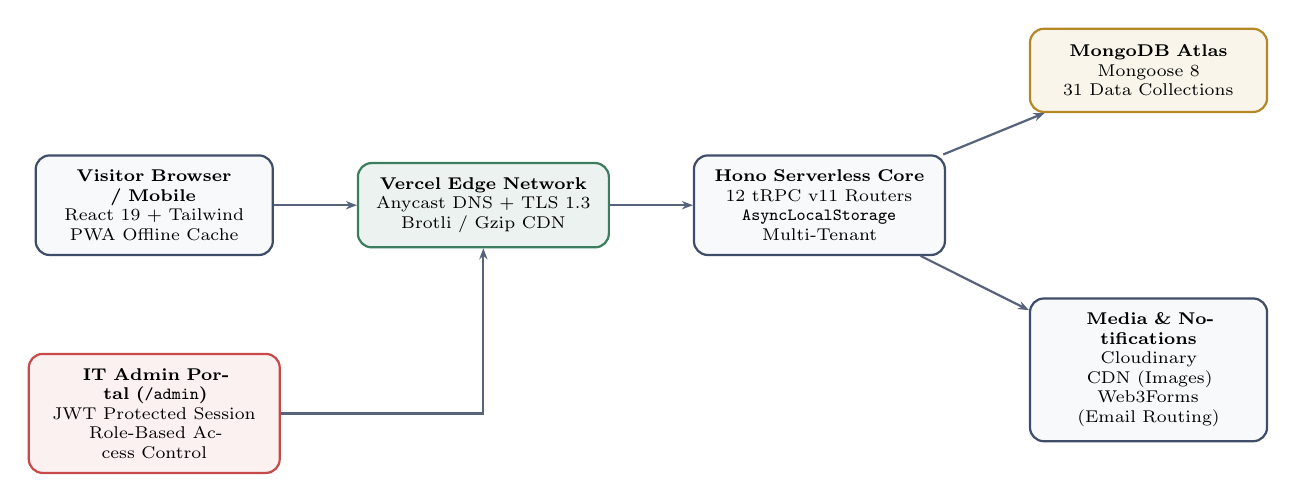
\begin{tikzpicture}[
  scale=0.88, every node/.style={transform shape},
  box/.style={rectangle, rounded corners=5pt, draw=dpsnavy!80, fill=codebg, thick, minimum height=1.2cm, align=center, font=\scriptsize, inner sep=6pt},
  edgebox/.style={box, draw=dpsgreen!80, fill=dpsgreen!8},
  dbbox/.style={box, draw=dpsgold!90!black, fill=dpsgold!10},
  arr/.style={-{Stealth[length=4pt]}, thick, draw=dpsnavy!70}
]

  \node[box, text width=3.0cm] (client) at (0, 0) {
    \textbf{Visitor Browser / Mobile}\\
    React 19 + Tailwind\\
    PWA Offline Cache
  };

  \node[edgebox, text width=3.2cm, right=1.2cm of client] (edge) {
    \textbf{Vercel Edge Network}\\
    Anycast DNS + TLS 1.3\\
    Brotli / Gzip CDN
  };

  \node[box, text width=3.2cm, right=1.2cm of edge] (api) {
    \textbf{Hono Serverless Core}\\
    12 tRPC v11 Routers\\
    \texttt{AsyncLocalStorage} Multi-Tenant
  };

  \node[dbbox, text width=3.0cm, above right=0.6cm and 1.2cm of api] (db) {
    \textbf{MongoDB Atlas}\\
    Mongoose 8\\
    31 Data Collections
  };

  \node[box, text width=3.0cm, below right=0.6cm and 1.2cm of api] (media) {
    \textbf{Media \& Notifications}\\
    Cloudinary CDN (Images)\\
    Web3Forms (Email Routing)
  };

  \node[box, text width=3.2cm, below=1.4cm of client, draw=alertred!80, fill=alertred!6] (admin) {
    \textbf{IT Admin Portal (\texttt{/admin})}\\
    JWT Protected Session\\
    Role-Based Access Control
  };

  \draw[arr] (client) -- (edge);
  \draw[arr] (edge) -- (api);
  \draw[arr] (api) -- (db);
  \draw[arr] (api) -- (media);
  \draw[arr] (admin) -| (edge);

\end{tikzpicture}
\caption{End-to-End DPSI Platform Operational and Governance Topology}
\label{fig:it-architecture}
\end{figure}

% ============================================================================
%  CHAPTER 2 — MASTER CREDENTIALS & ENVIRONMENT MATRIX
% ============================================================================
\chapter{Master Credentials \texorpdfstring{\&}{and} Environment Matrix}

\section{Environment Variable Reference Table}

The application relies on 12 environment variables configured within Vercel's
Environment Variables dashboard (or local \texttt{.env} file during testing).
Table~\ref{tab:env-matrix} provides the definitive configuration matrix.

\begin{table}[H]
\centering
\caption{Master Environment Variables and Security Classifications}
\label{tab:env-matrix}
\begin{tabularx}{\textwidth}{L{4.0cm} C{2.2cm} L{3.5cm} X}
\toprule
\textbf{Variable Name} & \textbf{Classification} & \textbf{Permitted Scope} & \textbf{Operational Purpose \& Guidance} \\
\midrule
\envvar{MONGODB\_URI} & \textcolor{alertred}{\textbf{Critical Secret}} & Server-side only & Primary MongoDB Atlas connection string including replica set, database name, and credentials. \\
\envvar{JWT\_SECRET} & \textcolor{alertred}{\textbf{Critical Secret}} & Server-side only & 64-character cryptographic entropy key used to sign and verify admin session tokens. \\
\envvar{ADMIN\_PASSWORD} & \textcolor{alertred}{\textbf{Critical Secret}} & Server-side only & Initial master password for the fallback root administrator account. \\
\envvar{ADMIN\_USERNAME} & Confidential & Server-side only & Root administrator account username (defaults to \texttt{admin}). \\
\envvar{DEV\_CREDIT\_UNLOCK\_PASSWORD} & \textcolor{alertred}{\textbf{Critical Secret}} & Server-side only & Secondary security password required to toggle developer attribution in the CMS. \\
\envvar{WEB3FORMS\_ACCESS\_KEY} & Confidential & Server-side only & Access key powering automated submission routing for the Contact and Admissions forms. \\
\envvar{CLOUDINARY\_CLOUD\_NAME} & Public / App & Server \& Client & Cloudinary account identifier for image hosting. \\
\envvar{CLOUDINARY\_API\_KEY} & Confidential & Server-side only & API key used for authorized image uploads and transformations. \\
\envvar{CLOUDINARY\_API\_SECRET} & \textcolor{alertred}{\textbf{Critical Secret}} & Server-side only & Cryptographic signing secret for Cloudinary asset deletion and folder sync. \\
\envvar{GEMINI\_API\_KEY} & Confidential & Server-side only & Google AI Studio key for the automated conversational counselor. \\
\envvar{ELEVENLABS\_API\_KEY} & Confidential & Server-side only & Neural voice synthesis API key for generating interactive audio responses. \\
\envvar{SENTRY\_DSN} & Public / App & Server \& Client & Telemetry endpoint for capturing client-side and server-side runtime exceptions. \\
\bottomrule
\end{tabularx}
\end{table}

\section{Rules for Managing Production Secrets}

\begin{itemize}[leftmargin=*]
  \item \textbf{Zero Hardcoding:}\ Never commit plaintext passwords, connection strings,
        or private keys to version control repositories.
  \item \textbf{Production Isolation:}\ Development, staging, and production environments
        must use separate MongoDB Atlas databases and separate Cloudinary folders.
  \item \textbf{Immediate Rotation on Breach:}\ If any key is inadvertently exposed in logs
        or client bundles, execute the \textit{Emergency Key Rotation Runbook} (Section~\ref{sec:sop-key-rotation}) immediately.
\end{itemize}

% ============================================================================
%  CHAPTER 3 — ACCESS CONTROL, AUTHENTICATION & SECURITY
% ============================================================================
\chapter{Access Control, Authentication \texorpdfstring{\&}{and} Security}

\section{Accessing the Administrative CMS Portal}

The administrative management suite is accessible at:
\begin{center}
  \url{https://dpsindirapuram.com/admin} \quad \textnormal{or} \quad \url{https://dpsindirapuram.com/admin/login}
\end{center}

\subsection{Login Credentials and Tenant Identification}

To authenticate successfully, the administrator must provide three fields:
\begin{enumerate}
  \item \textbf{Username:} Configured administrator username (e.g., \texttt{admin} or assigned staff handle).
  \item \textbf{Password:} Master administrator password (minimum 8 characters with alphanumeric requirements).
  \item \textbf{School Identifier Code:} \texttt{DPSI} (Enforces multi-tenant workspace routing in \texttt{AsyncLocalStorage}).
\end{enumerate}

\section{Dual-Layer Brute-Force Rate Limiter}

To safeguard the school from credential-stuffing attacks and brute-force cracking,
the platform enforces a coordinated two-tier lockout mechanism in \texttt{server/cms-router.ts}:

\begin{figure}[H]
\centering
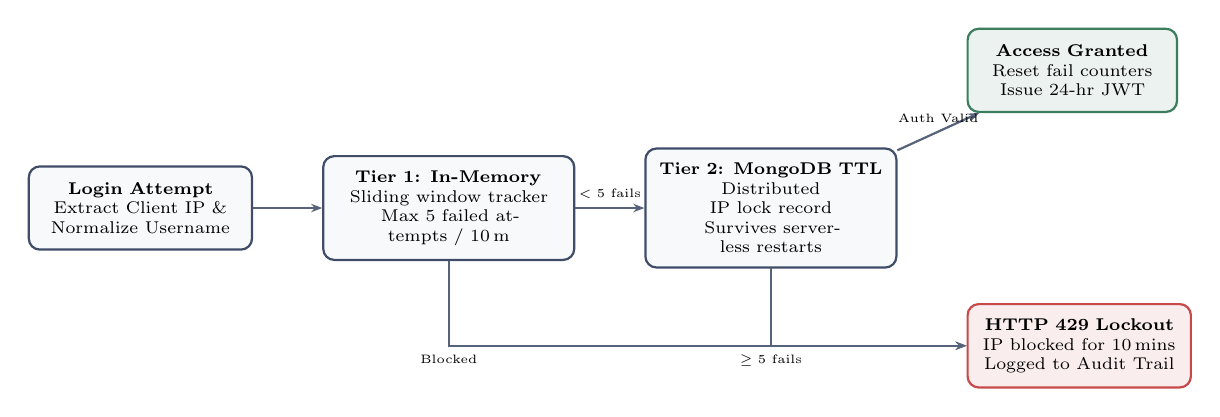
\begin{tikzpicture}[
  scale=0.88, every node/.style={transform shape},
  stepbox/.style={rectangle, rounded corners=4pt, draw=dpsnavy!80, fill=codebg, thick, minimum height=1.2cm, align=center, font=\scriptsize, inner sep=6pt},
  warnbox/.style={stepbox, draw=alertred!80, fill=alertred!8},
  passbox/.style={stepbox, draw=dpsgreen!80, fill=dpsgreen!8},
  arr/.style={-{Stealth[length=4pt]}, thick, draw=dpsnavy!70}
]

  \node[stepbox, text width=2.8cm] (attempt) at (0, 0) {
    \textbf{Login Attempt}\\
    Extract Client IP \&\\
    Normalize Username
  };

  \node[stepbox, text width=3.2cm, right=1.0cm of attempt] (tier1) {
    \textbf{Tier 1: In-Memory}\\
    Sliding window tracker\\
    Max 5 failed attempts / 10\,m
  };

  \node[stepbox, text width=3.2cm, right=1.0cm of tier1] (tier2) {
    \textbf{Tier 2: MongoDB TTL}\\
    Distributed IP lock record\\
    Survives serverless restarts
  };

  \node[passbox, text width=2.6cm, above right=0.5cm and 1.0cm of tier2] (success) {
    \textbf{Access Granted}\\
    Reset fail counters\\
    Issue 24-hr JWT
  };

  \node[warnbox, text width=2.8cm, below right=0.5cm and 1.0cm of tier2] (lockout) {
    \textbf{HTTP 429 Lockout}\\
    IP blocked for 10\,mins\\
    Logged to Audit Trail
  };

  \draw[arr] (attempt) -- (tier1);
  \draw[arr] (tier1) -- node[above, font=\tiny] {$<5$ fails} (tier2);
  \draw[arr] (tier2) -- node[above, font=\tiny] {Auth Valid} (success);
  \draw[arr] (tier2) |- node[below, font=\tiny] {$\ge 5$ fails} (lockout);
  \draw[arr] (tier1) |- node[below, font=\tiny] {Blocked} (lockout);

\end{tikzpicture}
\caption{Dual-Layer Rate Limiting Architecture Protecting Admin Endpoint}
\label{fig:rate-limiter}
\end{figure}

\subsection{Lockout Recovery Procedure}

If an authorized IT staff member is locked out after accidental mistypes:
\begin{enumerate}
  \item Wait \textbf{10 minutes} for the automatic TTL cooldown to expire.
  \item Or, connect via alternative network/IP (e.g., mobile hotspot) if access is urgent.
  \item In emergency circumstances, execute the database IP-unlock command described in Chapter~\ref{chap:sop}.
\end{enumerate}

\section{Developer Attribution Security Lock}

Per institutional guidelines, the developer attribution badge in the footer is protected
by a secondary authorization barrier. Toggling or editing attribution requires:
\begin{enumerate}
  \item Active Administrator session.
  \item Entry of the \envvar{DEV\_CREDIT\_UNLOCK\_PASSWORD} in the attribution modal dialog.
  \item A permanent audit record is created immediately upon successful or unsuccessful unlock attempts.
\end{enumerate}

% ============================================================================
%  CHAPTER 4 — CONTENT MANAGEMENT SYSTEM (CMS) OPERATIONAL MANUAL
% ============================================================================
\chapter{Content Management System (CMS) Operational Manual}

The DPSI CMS portal comprises \textbf{28 modular management engines}. This chapter provides
step-by-step instructions for operating every subsystem.

\section{High-Priority Broadcast: Emergency Marquee Ticker}

\textbf{Module Navigation:} CMS Sidebar $\rightarrow$ \texttt{Marquee / Notices}

The top announcement ticker is the primary channel for broadcasting high-priority alerts
(e.g., weather emergencies, winter timings, pollution holidays, or urgent transport reroutes).

\begin{enumerate}
  \item Click \textbf{``Create Announcement''}.
  \item Enter the notice text clearly in English (and Hindi if bilingual broadcast is required).
  \item Set \textbf{Priority} to \textit{High / Urgent} (renders with gold/red pulse animation).
  \item Set \textbf{Status} to \textit{Active}.
  \item Provide an optional external link or circular PDF attachment.
  \item Click \textbf{``Publish Announcement''}. The marquee updates globally on all client screens within 5 seconds without requiring page reloads.
\end{enumerate}

\section{Promotional Popups \& Admissions Modals}

\textbf{Module Navigation:} CMS Sidebar $\rightarrow$ \texttt{Popups}

Popups display prominent graphic overlays to announce annual admissions openings or major school events.

\begin{enumerate}
  \item Enter \textbf{Modal Title} and \textbf{Headline}.
  \item Upload the promotional creative image via the Cloudinary uploader (recommended aspect ratio: 4:3 or 16:9, max file size: 1.5\,MB).
  \item Configure \textbf{Call to Action (CTA) Button} label (e.g., \textit{``Apply for Nursery 2026--27''}) and target URL (e.g., \texttt{/admissions}).
  \item Configure \textbf{Display Trigger}:
        \begin{itemize}
          \item \textit{Once per Session:} Displays on initial visit, then respects user dismissal for 24 hours.
          \item \textit{Always Show:} Forces modal appearance on every page refresh (use only for mandatory institutional notices).
        \end{itemize}
  \item \textbf{Performance Safeguard:} The client application automatically defers modal hydration by \textbf{7.5 seconds} on mobile devices to preserve Core Web Vitals (LCP and TBT). Do not attempt to bypass this timeout in the codebase.
\end{enumerate}

\section{Admissions Pipeline \& Inquiries Management}

\textbf{Module Navigation:} CMS Sidebar $\rightarrow$ \texttt{Admission Steps} \textbar\ \texttt{Contact Messages}

\begin{enumerate}
  \item \textbf{Reviewing Applications:} Open \texttt{Contact Messages} to view real-time inquiries submitted via the web portal.
  \item \textbf{Triage Statuses:} Update inquiry status systematically:
        \begin{itemize}
          \item \rolebadge{linkblue}{New Inquiry} --- Newly ingested form submission awaiting review.
          \item \rolebadge{dpsgold}{Contacted} --- Admissions counselor has reached out via call/email.
          \item \rolebadge{successgrn}{Enrolled} --- Registration fee paid and seat allotted.
          \item \rolebadge{gray}{Archived / Invalid} --- Incomplete or duplicate submission.
        \end{itemize}
  \item \textbf{Exporting Data:} Click \textbf{``Export to CSV / Excel''} to download the current batch for upload into the DPS Indirapuram Administrative ERP.
\end{enumerate}

\section{Transfer Certificate (TC) Verification Engine}

\textbf{Module Navigation:} CMS Sidebar $\rightarrow$ \texttt{TC Verification}

CBSE regulations require schools to provide a public portal for verifying student Transfer Certificates.

\begin{enumerate}
  \item \textbf{Uploading New TC Record:}
        \begin{itemize}
          \item Enter \textbf{Admission Number}, \textbf{TC Number}, and \textbf{Student Name}.
          \item Select \textbf{Date of Issue}, \textbf{Class Last Studied}, and \textbf{Reason for Leaving}.
          \item Upload the digitally signed or scanned TC document (PDF format only, $\leq$2\,MB).
          \item Click \textbf{``Save \& Publish TC''}.
        \end{itemize}
  \item \textbf{Verifying Public Search:} Visit \url{https://dpsindirapuram.com/tc-search}, enter the student admission number, and confirm that the certificate renders and is downloadable.
\end{enumerate}

\section{Academic Circulars, Syllabi \& CBSE Mandatory Disclosures}

\textbf{Module Navigation:} CMS Sidebar $\rightarrow$ \texttt{Attachments}

\begin{enumerate}
  \item Click \textbf{``Upload Attachment''}.
  \item Select the target category:
        \begin{itemize}
          \item \textit{CBSE Mandatory Disclosure} (Affiliation grant letter, Society registration, NOC, Fire Safety certificate, Building Safety certificate).
          \item \textit{Fee Structure} (Annual tuition schedules, transport charges).
          \item \textit{Academic Syllabus \& Booklist} (Class-wise curated curricula).
          \item \textit{Examination Schedules \& Date Sheets}.
        \end{itemize}
  \item Attach the approved PDF file. The system automatically verifies that the document contains no executable payloads and generates a secure CDN permalink.
\end{enumerate}

\section{360° Virtual VR Tour Engine Management}

\textbf{Module Navigation:} CMS Sidebar $\rightarrow$ \texttt{VR Tour / Facilities}

The 3D virtual tour enables visitors to explore the 10-acre DPS Indirapuram campus
through spherical equirectangular panoramic projections.

\begin{enumerate}
  \item \textbf{Adding a Campus Node / Location:}
        \begin{itemize}
          \item Upload an \textbf{8192$\times$4096} or \textbf{4096$\times$2048} equirectangular 360$^\circ$ photograph.
          \item Label the node (e.g., \textit{``Senior Science Complex'', ``Olympic-Sized Swimming Pool'', ``Atrium''}).
        \end{itemize}
  \item \textbf{Placing Interactive Hotspots:}
        \begin{itemize}
          \item Use the visual placement tool to position Raycaster click coordinates $(\theta, \phi)$ in spherical space.
          \item Configure hotspot type: \textit{Navigation Target} (moves visitor to another scene) or \textit{Info Card} (displays laboratory specifications, teacher profiles, or student achievements).
        \end{itemize}
\end{enumerate}

\section{AI Admissions Assistant \& Voice Settings}

\textbf{Module Navigation:} CMS Sidebar $\rightarrow$ \texttt{AI Settings}

The AI chatbot uses Google Gemini 2.0 Flash for reasoning and ElevenLabs for voice synthesis.

\begin{enumerate}
  \item \textbf{Grounding Knowledge Base Updates:}
        \begin{itemize}
          \item Edit the institutional context block to update current school session fee brackets, age cut-off dates, bus routes, or uniform requirements.
          \item \textbf{Guardrail Directive:} The prompt includes strict instructions barring the AI from guessing fee waivers or admissions promises. Review system prompts quarterly.
        \end{itemize}
  \item \textbf{Voice Synthesis Controls:}
        \begin{itemize}
          \item Toggle voice playback on or off.
          \item Select ElevenLabs Voice ID (default: warm institutional counselor profile).
          \item Audio responses are automatically cached in MongoDB to prevent redundant API charges.
        \end{itemize}
\end{enumerate}

\section{Audit Logs \& System Observability}

\textbf{Module Navigation:} CMS Sidebar $\rightarrow$ \texttt{Audit Logs}

Every administrative mutation is recorded immutably with timestamp, actor username,
client IP address, affected resource ID, and operational diff.
IT administrators must inspect this log weekly for suspicious activity.

% ============================================================================
%  CHAPTER 5 — EMAIL INFRASTRUCTURE & WEB3FORMS PIPELINE
% ============================================================================
\chapter{Email Infrastructure \texorpdfstring{\&}{and} Web3Forms Pipeline}

\section{Architectural Design of Zero-Maintenance Email Bridge}

To eliminate SMTP server vulnerabilities, spam reputation degradation, and credential
leakage, all website contact forms and admissions inquiries route through
a hardened serverless bridge powered by \textbf{Web3Forms}:

\begin{equation}
  \text{User Form} \xrightarrow{\text{HTTPS POST}} \text{Hono Edge Server}
  \xrightarrow{\text{Zod Sanitization}} \text{Web3Forms API}
  \xrightarrow{\text{TLS SMTP}} \text{DPSI Admissions Desk Inbox}
\end{equation}

\section{Configuration and Key Verification}

The primary access key is stored securely in \envvar{WEB3FORMS\_ACCESS\_KEY}.
The CMS provides an administrative diagnostic tool in \texttt{CMS Sidebar $\rightarrow$ Site Settings}:

\begin{enumerate}
  \item Navigate to the \textbf{Web3Forms Integration} card in Site Settings.
  \item Click \textbf{``Send Diagnostic Test Email''}.
  \item The server executes a dry-run test submission.
  \item Verify that a test payload arrives at \texttt{admissions@dpsindirapuram.com} within 60 seconds.
\end{enumerate}

\section{Emergency Email Fallback Protocol}

If Web3Forms experiences external third-party outages:
\begin{itemize}
  \item Form submissions are \textbf{never lost}: the serverless router simultaneously
        persists the raw inquiry to the MongoDB \texttt{ContactMessage} collection.
  \item The IT Admin can view, triage, and export all submitted records directly from
        the \texttt{Contact Messages} tab in the CMS.
\end{itemize}

% ============================================================================
%  CHAPTER 6 — DATABASE MANAGEMENT & BACKUP PROTOCOLS
% ============================================================================
\chapter{Database Management \texorpdfstring{\&}{and} Backup Protocols}

\section{Database Topology (MongoDB Atlas)}

The production database is hosted on MongoDB Atlas in the \texttt{ap-south-1} (Mumbai, India)
AWS region for lowest latency to Delhi NCR visitors.
Connection pooling is managed by Mongoose with the following baseline parameters:
\begin{itemize}
  \item \texttt{maxPoolSize = 50}
  \item \texttt{minPoolSize = 5}
  \item \texttt{serverSelectionTimeoutMS = 5000}
  \item \texttt{socketTimeoutMS = 45000}
\end{itemize}

\section{Automated Backup Schedule}

MongoDB Atlas provides automated continuous data protection:
\begin{itemize}
  \item \textbf{Continuous Snapshots:} Hourly differential backups retained for 7 days.
  \item \textbf{Daily Master Snapshots:} Created at 02:00 IST every morning, retained for 30 days.
  \item \textbf{Point-in-Time Recovery (PITR):} Granular recovery to any millisecond within the past 7 days.
\end{itemize}

\section{Manual Backup \& Export Runbook}

IT staff must execute a manual cold backup prior to executing major database schema migrations
or major academic year rollovers:

\begin{lstlisting}[language=bash, caption={Manual Database Export Command}]
# Create full encrypted compressed dump of production database
mongodump --uri="mongodb+srv://dpsi_admin:<PASSWORD>@cluster0.mongodb.net/dpsi" \
          --gzip --archive=DPSI_DB_BACKUP_$(date +%Y%m%d).gz

# Verify backup archive integrity
ls -lh DPSI_DB_BACKUP_*.gz
\end{lstlisting}

\section{Restoration Runbook}

In the catastrophic event of malicious data destruction or database corruption:

\begin{lstlisting}[language=bash, caption={Database Restoration Command}]
# Restore archive to staging or disaster recovery cluster
mongorestore --uri="mongodb+srv://dpsi_admin:<PASSWORD>@cluster0.mongodb.net/dpsi" \
             --gzip --archive=DPSI_DB_BACKUP_20260917.gz --drop
\end{lstlisting}

% ============================================================================
%  CHAPTER 7 — MEDIA ASSETS & CDN MANAGEMENT
% ============================================================================
\chapter{Media Assets \texorpdfstring{\&}{and} CDN Management}

\section{Cloudinary Asset Architecture}

All photographs, banners, event galleries, and faculty portraits are served
via Cloudinary's multi-cloud edge CDN.
Assets are organized under the \texttt{dpsi-school/} root folder hierarchy:
\begin{itemize}
  \item \texttt{dpsi-school/gallery/} --- High-resolution event photographs.
  \item \texttt{dpsi-school/faculty/} --- Official staff portrait directory.
  \item \texttt{dpsi-school/sliders/} --- Homepage hero banners (1920$\times$1080).
  \item \texttt{dpsi-school/attachments/} --- Public documents and circulars.
\end{itemize}

\section{Automatic Optimisation Rules}

The application automatically enforces next-generation compression upon delivery:
\begin{itemize}
  \item Format negotiation: Serves \textbf{AVIF} to modern Chromium/Safari browsers, falling back to \textbf{WebP}.
  \item Quality optimization: \texttt{f\_auto,q\_auto:good} reduces average payload size by 65--80\,\%.
  \item Client-side pre-compression: Photos uploaded via CMS are compressed to $\leq$1\,MB before network dispatch.
\end{itemize}

% ============================================================================
%  CHAPTER 8 — CYBERSECURITY, COMPLIANCE & HARDENING
% ============================================================================
\chapter{Cybersecurity, Compliance \texorpdfstring{\&}{and} Hardening}

\section{OWASP Top 10 Security Posture}

The DPS Indirapuram digital platform achieved a \textbf{Grade A (96/100)} rating
during automated security penetration auditing. Table~\ref{tab:owasp-controls} details
the active defense controls.

\begin{table}[H]
\centering
\caption{OWASP Security Controls and Defense Implementation}
\label{tab:owasp-controls}
\begin{tabularx}{\textwidth}{L{4.2cm} L{3.5cm} X}
\toprule
\textbf{Vulnerability Category} & \textbf{Defense Mechanism} & \textbf{Implementation Details in Codebase} \\
\midrule
Injection (SQL / NoSQL) & Zod Schemas + Mongoose & Strong typing on all 12 tRPC routers. Rejection of unvalidated \texttt{\$where} or query operators. \\
Broken Authentication   & JWT + IP Rate Limiting  & Cryptographic token verification. 10-minute brute force lockout on 5 consecutive failures. \\
Sensitive Data Exposure & HTTPS Everywhere + HSTS & TLS 1.3 enforced. Passwords hashed using one-way cryptographic algorithms. \\
Security Misconfiguration & Security Response Headers & \texttt{X-Content-Type-Options: nosniff}, \texttt{X-Frame-Options: SAMEORIGIN}, strict CSP. \\
Cross-Site Scripting (XSS) & React DOM Sanitization & DOMPurify on RichText content. Automatic HTML entity encoding across all templates. \\
Vulnerable Dependencies & Automated Vulnerability Audit & Zero known vulnerabilities across all 73 production npm packages. \\
\bottomrule
\end{tabularx}
\end{table}

\section{Statutory Compliance Mandates}

\subsection{CBSE Mandatory Disclosure Norms}
The IT Administrator must ensure the \textbf{Mandatory Public Disclosure} page
remains active 24/7 at \url{https://dpsindirapuram.com/mandatory-disclosure} with
valid, unexpired PDF links for society registration, fire certificates, and water quality reports.

\subsection{Digital Personal Data Protection (DPDP) Act 2023}
\begin{itemize}
  \item All student photographs displayed on the website must have documented parent consent on file.
  \item Parent contact inquiry details stored in \texttt{ContactMessage} must be permanently purged or anonymized after 12 months.
\end{itemize}

% ============================================================================
%  CHAPTER 9 — STANDARD OPERATING PROCEDURES (SOPS)
% ============================================================================
\chapter{Standard Operating Procedures (SOPs) \texorpdfstring{\&}{and} Runbooks}
\label{chap:sop}

\section{SOP 1: Emergency Weather or Pollution School Closure Broadcast}

\sopbox{SOP 1 --- Target Execution Time: Under 2 Minutes}{
  \textbf{Trigger:} District Magistrate / Directorate of Education announces sudden school closure due to heavy rain, extreme cold, or air pollution.\\[3pt]
  \textbf{Step 1:} Open \url{https://dpsindirapuram.com/admin} on desktop or mobile.\\[2pt]
  \textbf{Step 2:} Log in and navigate to \textbf{Marquee / Notices}.\\[2pt]
  \textbf{Step 3:} Click \textbf{``Add Notice''}, type the official closure circular summary (e.g., \textit{``As per DM order, school will remain closed for Classes Nursery--VIII on 18 Sept 2026. Online classes will operate via MS Teams.''}).\\[2pt]
  \textbf{Step 4:} Set Priority to \textbf{Urgent}, Status to \textbf{Active}.\\[2pt]
  \textbf{Step 5:} Click \textbf{Publish}. Refresh homepage to verify ticker visibility.
}

\section{SOP 2: Master Administrator Password Reset}
\label{sec:sop-password}

\sopbox{SOP 2 --- Emergency Password Recovery}{
  \textbf{Scenario:} IT Admin forgot master password or suspect unauthorized access.\\[3pt]
  \textbf{Method A (Via CMS):} If currently logged in, go to \textbf{Site Settings} $\rightarrow$ \textbf{Change Password}, enter current and new password.\\[2pt]
  \textbf{Method B (Serverless Environment Override):}
  \begin{enumerate}[leftmargin=*]
    \item Open Vercel Project Dashboard $\rightarrow$ \textbf{Settings} $\rightarrow$ \textbf{Environment Variables}.
    \item Update \envvar{ADMIN\_PASSWORD} with a newly generated high-entropy secret.
    \item Trigger a redeployment via \textbf{Deployments} $\rightarrow$ \textbf{Redeploy}.
    \item The server will synchronize the new password to the root admin record.
  \end{enumerate}
}

\section{SOP 3: Annual Board Exam Results Release Day Preparation}

\sopbox{SOP 3 --- High-Traffic Event Readiness}{
  \textbf{Trigger:} CBSE Class X and Class XII board examination results release day.\\[3pt]
  \textbf{Action 1 (48 Hours Prior):} Log in to CMS $\rightarrow$ \textbf{Board Results} tab. Pre-format the topper banners and percentage distribution charts.\\[2pt]
  \textbf{Action 2 (Cache Verification):} Confirm Cloudflare / Vercel Edge caching is active to absorb 50,000+ concurrent parent visits.\\[2pt]
  \textbf{Action 3 (Hero Banner):} Publish congratulations banner with school topper photographs.\\[2pt]
  \textbf{Action 4 (Post-Release):} Verify that dynamic score lookup is performing at $<100$\,ms response time.
}

\section{SOP 4: Rotating Third-Party API Keys}
\label{sec:sop-key-rotation}

\sopbox{SOP 4 --- Quarterly Security Key Rotation}{
  \textbf{Frequency:} Every 90 days or immediately upon team departure.\\[3pt]
  \textbf{Step 1:} Generate new API keys in respective vendor dashboards (Web3Forms, Cloudinary, Gemini, ElevenLabs).\\[2pt]
  \textbf{Step 2:} Update environment variables in Vercel settings.\\[2pt]
  \textbf{Step 3:} Promote new deployment to production.\\[2pt]
  \textbf{Step 4:} Test all affected functionalities (Contact form submission, AI chatbot response, image upload).
}

% ============================================================================
%  CHAPTER 10 — DIAGNOSTICS, LOGGING & VENDOR CONTACTS
% ============================================================================
\chapter{Diagnostics, Logging \texorpdfstring{\&}{and} Vendor Directory}

\section{Running Automated System Diagnostics}

The IT team can verify platform health using the automated Vitest test suite:

\begin{lstlisting}[language=bash, caption={Executing Comprehensive Platform Health Test Suite}]
# Execute full system audit test suite (150 tests across 9 domains)
cd /Users/0xshashank/Documents/School\ Project/DPSI_Website/app
npx vitest run

# Expected Result:
# Test Files  9 passed (9)
# Tests       150 passed (150)
# Duration    < 2.5s
\end{lstlisting}

\section{Incident Escalation Matrix}

Table~\ref{tab:escalation} provides the incident escalation protocol for IT staff.

\begin{table}[H]
\centering
\caption{IT Incident Escalation and Service Provider Directory}
\label{tab:escalation}
\begin{tabularx}{\textwidth}{L{3.2cm} C{2.2cm} L{3.5cm} X}
\toprule
\textbf{Infrastructure Tier} & \textbf{Service Provider} & \textbf{Dashboard / Portal} & \textbf{Escalation Role \& Protocol} \\
\midrule
Web Hosting \& Edge CDN  & Vercel Inc. & \url{vercel.com/dashboard} & Primary host. Check status page (\url{vercel-status.com}) during routing failures. \\
Database Cluster         & MongoDB Atlas & \url{cloud.mongodb.com} & Inspect CPU spikes, connection pool limits, or replica failovers. \\
Media \& Image CDN       & Cloudinary & \url{cloudinary.com/console} & Bandwidth quotas, transform credits, and storage metrics. \\
Email Routing Bridge     & Web3Forms & \url{web3forms.com} & Form submission tracking and webhook delivery statuses. \\
Error Telemetry          & Sentry.io & \url{sentry.io} & Real-time inspection of unresolved client exceptions. \\
School IT Desk           & DPSI IT Team & \texttt{it@dpsindirapuram.com} & Internal on-call school systems administrator. \\
\bottomrule
\end{tabularx}
\end{table}

\vspace{1.5cm}
\begin{center}
  \rule{0.6\textwidth}{0.8pt}\\[0.2cm]
  \textbf{\textcolor{dpsnavy}{END OF OFFICIAL IT ADMINISTRATOR \& OPERATIONS MANUAL}}\\[0.1cm]
  \textit{Delhi Public School Indirapuram --- All Rights Reserved \textbar\ Confidential}
\end{center}

\end{document}
